\section*{摘要}
本研究用两个小规模案例，考察可执行反馈怎样指导语言模型系统的优化，以及怎样验证优化是否真正发生。第一个案例实现 LoRA 低秩适配，并以固定版本 OpenRLHF 对 \path{Qwen/Qwen2.5-0.5B} 进行 PPO 算术任务训练。独立的功能检查覆盖参数冻结、数值等价与合并；随后在 NVIDIA A10 上，以 BF16 完成 512 道训练题、32 个采样批次、适配器保存及 Actor 重载。同一组 128 道开发验证题的首行整数答案正确数由 117 增至 122，变化为 3.90625 个百分点。第二个案例在 LLM4AD\_Next 平台用真实模型调用搜索 26 圆布局程序，保存了 5 次有效在线评估，最佳在线半径和为 2.62001380699489；导出程序的独立本地复现另得 2.6206092130170973。两个数值来自不同记录，分别保留。研究未进行多随机种子或超参数消融；在线搜索手动停止，也未证明全局最优。本文的主要产出是可检查的实现、实验结果及证据链，而不是通用推理能力或新优化算法的证明。

{\small\color{muted}\key{关键词：}低秩适配；PPO；程序搜索；外部评估；实验复核。中文说明与英文报告采用相同数据和结论，另补充必要的概念解释。}

\section{引言与研究问题}
语言模型系统可以在不同层面接受反馈。一种方式是调整模型参数，使以后生成某种回答的概率发生变化；另一种方式是保留模型本身，通过反复生成、执行和筛选代码，改变最终使用的程序。前者的优化对象是参数，后者的优化对象是程序。两者都需要把“看起来合理”与“经过执行验证”分开。

本研究围绕两个具体问题展开：
\begin{enumerate}
\item 在小型算术任务上，能否完成从 LoRA 实现、PPO 训练，到保存、重载和同条件评估的可检查流程？实际任务分数怎样变化？
\item 在固定的几何约束和有限搜索记录中，大模型引导的程序搜索能否产生有效候选？在线分数和独立复现分别支持什么结论？
\end{enumerate}
这两个案例的任务、指标和预算不同，因此不是 LoRA-PPO 与程序搜索之间的优劣对比。共同考察的是反馈怎样进入系统、结果怎样测量，以及哪些额外检查能防止把过程日志误当成最终成功。

\begin{minipage}{\linewidth}
\par\noindent\begin{minipage}{\linewidth}
\begin{center}
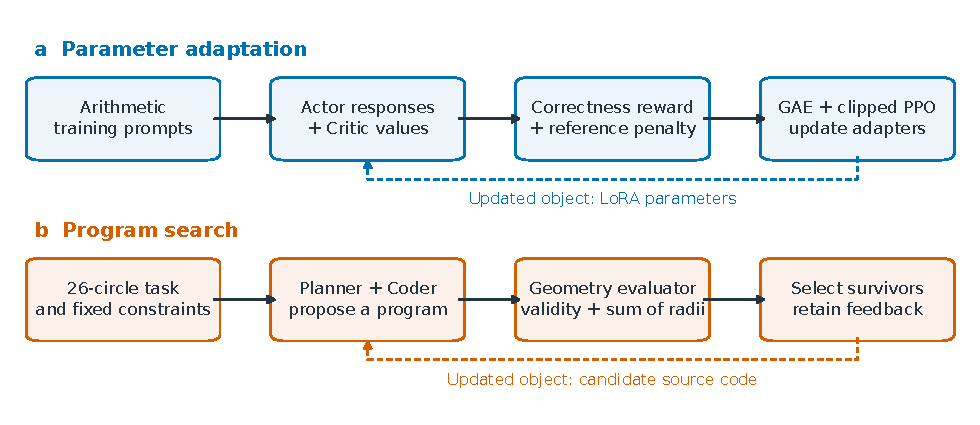
\includegraphics[width=166mm]{../../figures/feedback_mechanisms.pdf}
\end{center}
\figcaption{fig:feedback-zh}{两种反馈驱动优化的机制示意。参数适应改变 LoRA 参数，程序搜索改变候选代码；图用于解释研究设计，不是实验分数、平台截图或新增算法的证明。}
\end{minipage}\par

\end{minipage}

实施过程中，除了记录成功运行，也保留了早期模型保存失败、下载中断、运行保护和在线无效候选。正文先说明方法和设计，再报告已核实的结果；附录保留实现说明、历史保存失败、运行范围及复现索引。
